\chapter{Analyse}\label{ch:analyse}
Im Folgendem erfolgt eine Beschreibung der Beispielanwendung `Rechnungsschreibung`.
Die dafür benötigten Informationen stammen aus Gesprächen mit Mitarbeiter 1 aus der Abteilung, die für die Rechnungsschreibung zuständig ist.
Hierbei wird vor allem der technische Aspekt beleuchtet.
Anschließend wird der aktuelle Bereitstellungsprozess für Laufzeitumgebungen, den dazugehörigen Datenbanksystem und einer Messaging Lösung dargestellt.

\section{Rechnungsschreibung}
Für diese Arbeit wurde die Rechnungsschreibung als Beispielanwendung herangezogen, weil sie folgenden Anforderungen entspricht.
Es handelt sich zum einem um eine in sich abgeschlossene Anwendung, die nur zu Beginn des Prozesses von anderen Anwendungen abhängig ist.
Zum anderen benötigt die Rechnungsschreibung ein CICS als Laufzeitumgebung, eine Db2-Datenbank und MQ als Messaginglösung.
Somit kann ein umfangreicher Bereitstellungsmechanismus in dieser Arbeit untersucht werden.

\subsection{Beschreibung}\label{rechBesch}
Die Erzeugung der Rechnungen lässt sich in mehrere Schritte unterteilen, gesammelt werden diese Schritte als Rechnungsschreibung bezeichnet.\\
Bei dem Ablauf handelt es sich um einen Batch\footnote{Stapelverarbeitung}-Ablauf, der auf einem Großrechner läuft.
Nur die Preisermittlung wird in ein CICS ausgelagert.
Zunächst wird nach jeder kostenpflichtigen Leistungserbringung durch die dazugehörige Anwendung ein Berechnungssatz erzeugt.
Ein Berechnungssatz beinhaltet die Metainformationen der Berechnung unter anderem die Artikelnummer, Menge und den Ordnungsbegriff.
Der Preis und der Rechnungsempfänger wird zu einem späteren Zeitpunkt innerhalb der Rechnungsschreibung ermittelt.

\subsubsection{Einpflegung Berechnungssätze}
Für das Einpflegen der Berechnungssätze in den Rechnungsschreibungsablauf stehen den Anwendungen drei Möglichkeiten zur Verfügung. \\
Bei der Ersten Möglichkeit handelt es sich um die Verwendung des DMVINF\footnote{DatevMakroVerarbeitungsinformation}-Moduls und der dazugehörigen Schnittstelle.
Dieses Modul ist in der Programmiersprache Assembler entwickelt worden.
Das Ergebnis dieses Moduls ist eine sequenzielle Datei am Großrechner, dieses Format lässt sich mit einer .txt Datei unter Windows vergleichen.
Diese Datei, auch Berechnungsdatei genannt, hat folgenden Aufbau.
Der erste Satz enthält Steuerinformationen, wie zum Beispiel Datum/Uhrzeit, Produkt usw.
Danach kommen die eigentlichen Berechnungssätze.
Schließlich folgt noch die Anzahl der Sätze und die Summe der einzelnen Artikel in einem Satz mit Kontrollinformationen.
Diese Kontrollinformationen werden im weiteren Verlauf mit den eingelesenen Werten abgeglichen, dadurch wird Datenverlust und unkontrollierte Eingriffsmöglichkeiten von außen ausgeschlossen.
Aus dem Aufbau einer solchen Datei lässt schließen, dass verschiedene Schritte für die Erzeugung innerhalb der Anwendung notwendig sind.

Für die nachfolgenden Schritte stellt das DMVINF-Modul jeweils Schnittstellen zur Verfügung.
Zuerst wird beim sogenannten Open die Datei erstellt und der Steuersatz geschrieben.
Danach folgt das eigentliche Schreiben der Berechnungssätze, dabei dürfen nur bestimmte Felder (Ordnungsbegriffe, Länderschlüssel und Mengen) verändert werden.
Um unzulässige Veränderungen zu verhindert, haben diese einen Abbruch der Verarbeitung zur Folge.
Schließlich folgt noch der `Close` bei dem die Kontrollinformationen geschrieben werden.
Hinzuzufügen ist, dass die variablen Informationen einer Formalprüfung unterzogen werden.
So entstehen je nach fachlicher Logik und Laufhäufigkeit der Anwendung mehrere Berechnungsdateien.

Eine weitere Möglichkeit die Berechnungsinformationen in den Ablauf einzupflegen ist die Übergabe über einen mit der Programmiersprache Java realisierte WebService.
Hier werden die Berechnungsinformationen im XML-Format bereitgestellt.
Das Ergebnis der entsprechenden Plausibilitätsprüfungen, die in einem Onlineverfahren durchgeführt werden, wird direkt an die aufrufende Anwendung zurückgegeben.
Sind die Daten korrekt werden diese vorerst in einer Datenbank gespeichert.
Vor dem nächsten Schritt wird diese Datenbank ausgelesen und mit der ersten Möglichkeit in den Kernablauf eingespeist.

Bei der letzten Möglichkeit handelt es sich um die Übergabe mittels einer CSV-Datei.
Die Datei wird auf den Großrechner übertragen und dort mit dem DMVINF-Modul verarbeitet.
Dieses Verfahren wird kaum von produktiven Anwendungen sondern hauptsächlich für Test- oder Qualitätssicherungszwecke genutzt.

Mittels dieser drei Möglichkeiten werden insgesamt monatlich circa 30 Millionen Datensätze bereitgestellt und weiterverarbeitet.
Diese Datensätze stehen innerhalb der durch das DMVINF-Modul erzeugten Berechnungsdateien dem weiteren Verlauf als Input zur Verfügung.
Um sicher zu stellen, dass all diese Dateien auch verarbeitet werden, wird bei Erstellung einer solchen ein Eintrag in eine Kontrolldatei vorgenommen.
In dieser Kontrolldatei wird jedes Lesen und somit auch das Lesen im weiteren Verlauf gekennzeichnet.
Eine monatliche Überprüfung führt die zuständige Abteilung durch.

\subsubsection{Tägliche Bewertung}
Der nächste Schritt des Rechnungsschreibungsprozesses ist die sogenannte Tägliche Bewertung.
Dieser Ablauf läuft einmal täglich von Montag bis Freitag und ist für die Preis- und Rechnungsempfängerermittlung zuständig.
Zur Realisierung wurden die Programmiersprachen Assembler und COBOL genutzt.
Am Ende dieses Ablaufes steht die ARUBA\footnote{Abrechnungs- und Umsatz-Basis}-Db2-Datenbank.
Dort werden die Berechnungsdaten der letzten 36 Monate aufbewahrt.
Dabei handelt es ich um insgesamt circa 3,8 Milliarden Datensätze von einer Gesamtgröße von circa 400 GB mit Indizes.
Diese Datensätze beinhalten alle Informationen für die endgültige Erzeugung der Rechnungen.

Der erste Schritt der Täglichen Bewertung ist das Zusammenführen der Berechnungsdateien aus dem vorherigen Schritt und aus den bereits vorhandenen Daten des laufenden Monats aus der ARUBA-Db2-Datenbank.
Zusätzlich werden während dieser Zusammenführung den Berechnungssätzen auf Basis der abgebenden Anwendung die entsprechenden Rechnungsstellungsrythmen (täglich oder monatlich) zugewiesen.
Anschließend wird mit Hilfe der Beraternummer die zugehörigen Betriebsstätte-, Rechnungsempfänger-, Hauptberater- und Mitglieds- bzw. Geschäftspartnernummer ermittelt.
Die Beraternummer ist als oberster Ordnungsbegriff in den Berechnungssätzen enthalten.
Außerdem wird die Debitorenkontonummer entweder durch die Mitglieds- oder durch die Geschäftspartnernummer zugeordnet.
Für die Preisermittlung werden die Datensätze nach Geschäftspartner gruppiert.
Im DATEV eG Umfeld ist ein Geschäftspartner entweder eine Kanzlei oder ein einzelner Mandant, dieser ist jedoch meist einer Kanzlei zugeordnet.

Dann werden die gruppierten Daten auf Grund der Performance an ein CICS übertragen.
Die Architektur wird in \ref{rechArch} beschrieben.
Dort findet die Preisermittlung mit den dazugehörigen kundenindividuellen Abhängigkeiten, wie zum Beispiel Rabatte, statt.
Anschließend werden die Daten wieder zurück an den Batch-Ablauf übertragen.
Hier werden die Rechnungsnettobeträge geprüft, ob diese über einem bestimmten Rechnungslimitbetrag liegen.
Falls dies nicht der Fall ist, werden die Berechnungssätze als BUL\footnote{Berater unter Limit} gekennzeichnet und in die folgende Rechnungsperiode vorgetragen.
Schließlich wird noch die Umsatzsteuer ermittelt.
Abschließend werden die neu erzeugten Berechnungsdaten in die ARUBA-Db2-Datenbank eingepflegt und entsprechend gekennzeichnet.

\subsubsection{Rechnungsaufbereitung}
Als letzter Schritt folgt die Rechnungsaufbereitung.
Diese erfolgt am ersten Werktag im Monat.
Mit Hilfe der ARUBA-Db2-Datenbank wird ermittelt, welchen Kunden eine Rechnung zugestellt werden muss.
Außerdem wird dabei der Zustellungsweg, per Post oder E-Mail, bestimmt.
Darauf folgt die Aufbereitung der Druckrohdaten und letztlich das Versenden der Rechnungen an die Berater.
Zusätzlich werden die Rechnungen noch im PDF-Format archiviert.

\subsection{Architektur der Preisermittlung}\label{rechArch}
In dieser Arbeit steht das automatisierte Provisionieren von Laufzeitumgebungen im Fokus.
In diesem Fall handelt es sich um die Laufzeitumgebung CICS mit den dazugehörigen Elementen.
Deshalb wird im Folgenden nur darauf eingegangen.

Das System muss an Lasttagen bis zu 180.000 Geschäftspartner verarbeiten können.
Um all diese an das CICS zu übertragen stehen dem System mehrere IBM MQ Queues zur Verfügung.
Bevor die eigentliche Bestimmung der Preise stattfindet, werden zunächst die Listenpreise ermittelt.
Hierfür werden zwei Queues verwendet.
Eine startet eine Transaktion im CICS, die andere wartet auf deren Antwort.
In diesem Ablauf werden die benötigten Listenpreise aus einer Datenbank ausgelesen und in einen Hauptspeicherbereich der CICS Instanz gespeichert.
Dies ist auf Grund der Last auf dem System notwendig, da ein Hauptspeicherzugriff schneller als ein Datenbankzugriff ist.
Somit gab es bei der Laufzeit eine Einsparung um circa XXXX Prozent.

Für die Bestimmung der Preise mit den Preisabhängigkeiten bestehen weitere Queues.
Darunter ist eine allgemeine Queue in der alle Aufträge, die für die Weiterverarbeitung zur Verfügung stehen, geschrieben werden.
Pro Geschäftspartner wird ein Auftrag angelegt.
In diesem Auftrag befinden sich die Namen vier weiterer Queues.
Eine dieser Queues beinhaltet alle Informationen, die für die Preisermittlung des dazugehörigen Geschäftspartners notwendig sind.
In den restlichen drei Queues sind die Ergebnisse der Preisermittlung gespeichert.
Die Queuenamen werden nicht dynamisch generiert, da dies zu Performanceproblemen führt.
Deshalb existieren für jede der vier Queues jeweils 100 vorgefertigte Namen.
Somit können auch maximal nur 100 Aufträge gleichzeitig auf Weiterverarbeitung warten.
Falls dieses Limit erreicht ist, wartet der Batch-Ablauf solange bis einer der Aufträge fertig gestellt wird.
Sobald ein Auftrag in die allgemeinen Auftragsqueue geschrieben wird, wird eine CICS-Transaktionen gestartet.
Diese führt die Preisermittlung durch und schreibt das Ergebnis auf die dazugehörigen Queues.
Ist dies geschehen stehen die Queues wieder für einen neuen Auftrag zur Verfügung.
Es können maximal 30 Transaktionen zeitgleich arbeiten.

Für die Preisermittlung wird auch eine Db2-Datenbank, in der die Einzelpreise der Artikel gespeichert sind, verwendet.
Wenn alle Transaktionen direkt auf diese Datenbank zugreifen würden, hätte dies über 60 Millionen Datenbankzugriffe zur Folge.
Dies führt zu massiven Einbußen bei der Performance.
Deshalb werden bevor die eigentliche Preisermittlung stattfindet, alle benötigten Einzelpreise und Preisabhängigkeiten ermittelt.
Diese Informationen werden dann in einen sogenannten `SHARED GETMAIN`-Bereich gespeichert.
Dabei handelt es sich im Prinzip um einen Hauptspeicherbereich des Großrechners.
Die Adresse von diesem Bereich wird dem Ablauf zur Verfügung gestellt.
Somit greifen die einzelnen Transaktionen nicht mehr direkt auf die Datenbank zu, sondern auf den schnelleren Hauptspeicher.

\section{Aktueller Bereitstellungsprozess}
 \begin{figure}[h]
\centering
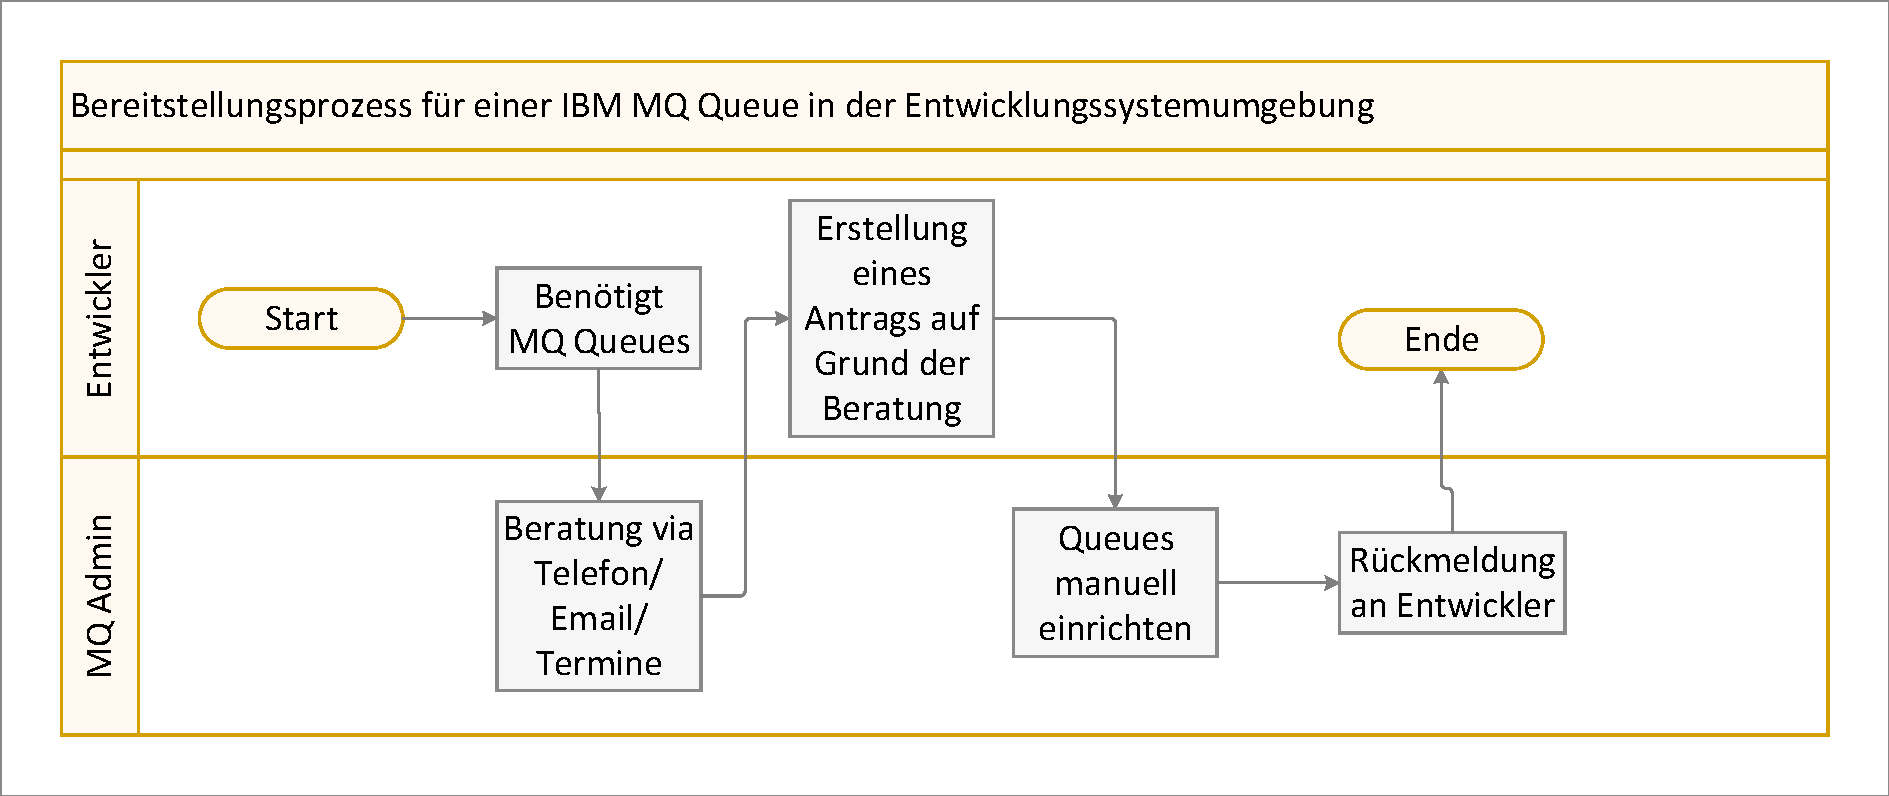
\includegraphics[width=\textwidth]{figures/swimlaneMQ.pdf}
\caption{Bereistellungsprozess von MQ}
\label{fig:aktmq}
\end{figure}

Mit vielen anderen Abteilungen sprechen\\
Viel auf `Zuruf` und Besprechungen\\
Genauere Infos noch von den CICSAdmins nachfragen\\

 